\RequirePackage{silence}
\WarningFilter{titlesec}{Non standard sectioning command detected}
\WarningFilter{scrartcl}{You've used obsolete option `onelinecaption'}
\WarningFilter{scrartcl}{Activating an ugly workaround for a missing}
\WarningFilter{scrartcl}{deprecated option `enabledeprecatedfontcommands'.}
\WarningFilter{scrartcl}{Usage of package `fancyhdr' together}
\WarningFilter{scrartcl}{Usage of package `titlesec' together}

\documentclass[paper=a4,nochapname,accentcolor=tud9c]{tudexercise}

\usepackage[english]{babel}
\usepackage{csquotes}
\usepackage[maxcitenames=2]{biblatex}
\addbibresource{References.bib}

\newcommand\textcitep[1]{\mkbibparens{\textcite{#1}}}
\newcommand\textcitesp[1]{\mkbibparens{\textcites{#1}}}

\usepackage[calc,useregional]{datetime2}
\newcount\mydatect
\newcount\datecount
\newcommand{\setdate}[1]{%
    \DTMsavedate{mydate}{#1}%
    \DTMmakeglobal{mydate}%
}%
\newcommand{\adddays}[1]{%
    \DTMsaveddateoffsettojulianday{mydate}{#1}{\mydatect}%
    \DTMsavejulianday{mydate}{\number\mydatect}%
    \DTMmakeglobal{mydate}%
}%

\usepackage{blindtext}
\usepackage{float}
\usepackage{tikz}
\usetikzlibrary{shapes.misc,arrows,positioning}

% https://tex.stackexchange.com/a/62273
\newenvironment{customlegend}[1][]{%
    \begingroup
    % inits/clears the lists (which might be populated from previous
    % axes):
    \csname pgfplots@init@cleared@structures\endcsname
    \pgfplotsset{#1}%
}{%
    % draws the legend:
    \csname pgfplots@createlegend\endcsname
    \endgroup
}%
\def\addlegendimage{\csname pgfplots@addlegendimage\endcsname}

\usepackage{hyperref}
\usepackage{enumitem}

\makeatletter
\def\namedlabel#1#2{\begingroup
    #1%
    \def\@currentlabel{\thedescriptcount}%
    \phantomsection\label{#2}\endgroup
}
\makeatother

\newcounter{descriptcount}
\newlist{enumdescript}{description}{2}
\setlist[enumdescript,1]{%
  before={\setcounter{descriptcount}{0}%
  \renewcommand*\thedescriptcount{[\Alph{descriptcount}]}}
  ,font=\bfseries\stepcounter{descriptcount}\thedescriptcount~%
}
\setlist[enumdescript,2]{%
  before={\setcounter{descriptcount}{0}%
          \renewcommand*\thedescriptcount{\roman{descriptcount}}}
  ,font=\bfseries\stepcounter{descriptcount}\thedescriptcount~
}

% Notes:
% Multi Party Session Types \subset Session Types \subset Behavioral Types

\title{Semi-Dynamic Session Types for ABS}
\subtitle{Bachelor Thesis Proposal, Software Engineering Group}
\subsubtitle{Anton Haubner}

%\raggedbottom
\begin{document}
%
\maketitle
%
\tableofcontents

\section{Motivation}
Reasoning about distributed systems which employ asynchronous interactions between their
components is usually difficult.
For example, one might want to ensure, that said components adhere to a specific
protocol, or that resources are properly allocated and released between uses.

When manually checking a model of a distributed system against a protocol
specification becomes too labor-intensive and time-consuming, automatic verification
can reduce the workload and help to avoid human errors.

Furthermore, if behavior can be dynamically added to the system during execution,
for instance by an interface of the runtime, the set of properties which
can be proven by static analysis of the system can become very limited.

Even in this case, some guarantees can still be enforced, if the schedulers of
asynchronous processes are aware of a protocol and only schedule those tasks
which do not violate it.

\paragraph{Thesis Topic}

The Abstract Behavioral Specification language (ABS) is intended for modeling
``distributed, object-oriented'' software systems \textcitep{johnsen2010abs} and
aims for ``verifiable design'' \textcitep{hahnle2012abstract} via a suite of external tools.

This thesis is based on % TODO: "new" correct? Really not mentioning authors of central source by name?
\textcitesp{kamburjan2018stateful, kamburjan2016session} and
aims at developing a tool for automatically verifying whether objects within an
ABS software model comply with a communication protocol, which is specified
using Session Types.

Furthermore, it will extend all participating objects with a scheduler \textcitep{bjork2013user} which
ensures, that only those processes are activated that the protocol permits to execute.
This is necessary, since the ABS Model API \textcitep{schlatte2018release} allows to asynchronously call methods during
runtime, which will invalidate static verification.
This idea has been explored in \textcitep{kamburjan2016session}.

\textcite{kamburjan2018stateful} also introduce Async Dynamic Logic (ADL) such that ADL formulas can
accompany protocol specifications and allow to express logical constraints on the
program state before method invocations and after their termination.
Although automatic verification of those constraints could  be implemented using
KeY-ABS \textcitep{din2015key}, it will likely exceed the time available for
implementing the thesis.
Instead, those constraints will optionally be implemented as runtime assertions,
if time allows.

\section{Working Packages}\label{workpackages}
%
\begin{figure}[H]
  \centering
  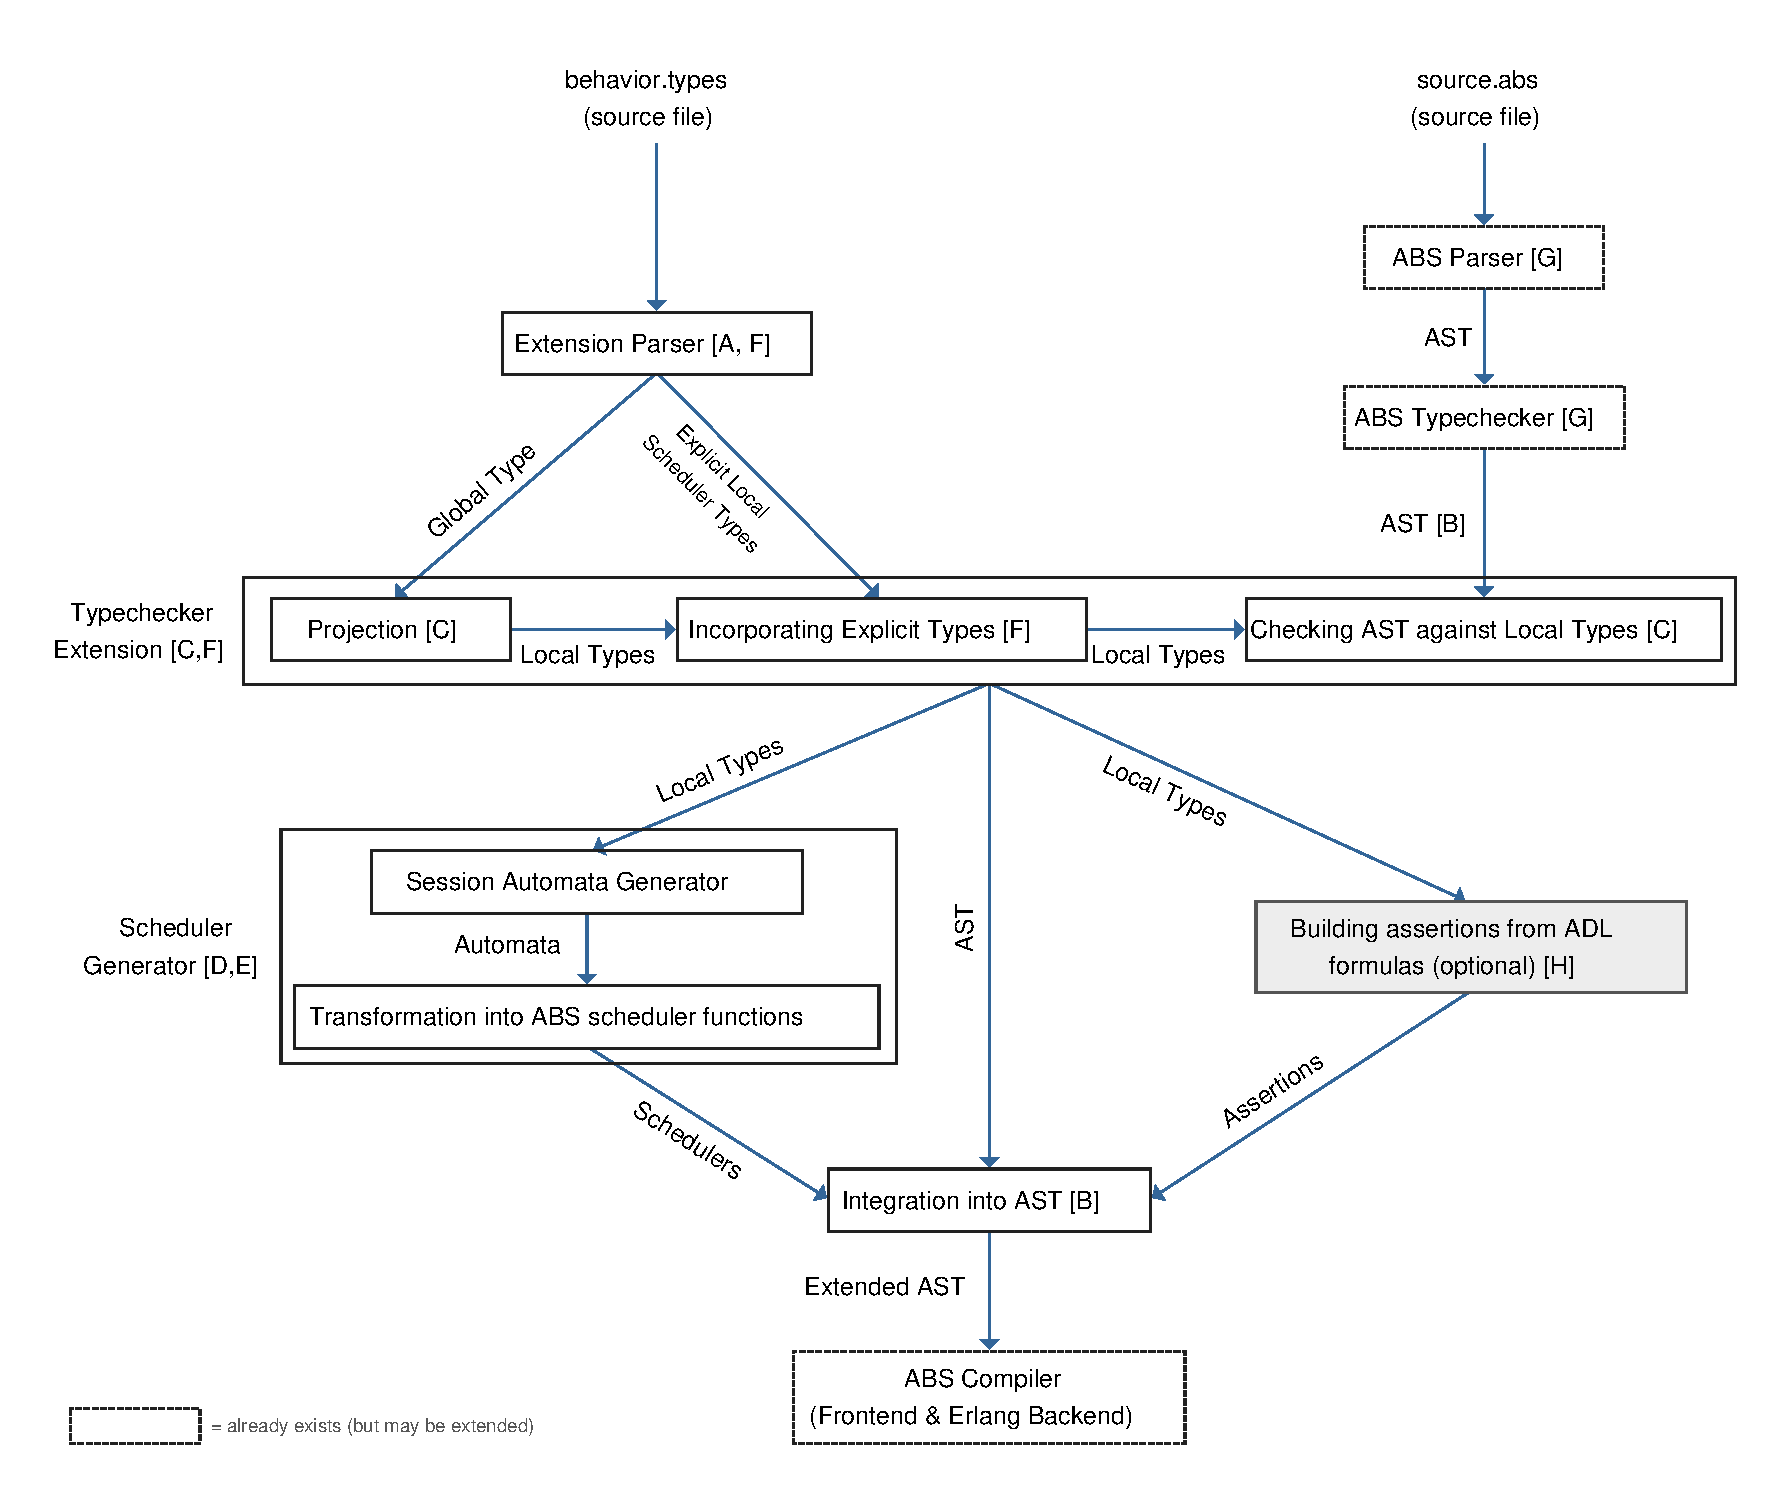
\includegraphics[width=\linewidth]{assets/architecture.pdf}
  \caption{Expected internal structure of the verification tool. The approximate scope of the working packages has been annotated using the [$\cdot$] notation.}
\end{figure}

All of the following working packages include a time investment proportional to the
complexity of the package, which is reserved for conducting the necessary
research using papers relevant to the topic. Also some time will be required for
detailed planning of the implementation of the package and recording the results
within the thesis document.

\begin{enumdescript}
\item[\namedlabel{Session Types syntax \& parser}{WPsyntaxAndParser}]%
    The verification tool which is to be developed during the thesis will require
    an input source where developers can define their protocol specifications using a variant of Session Types.

    Coupling between the ABS compiler and the verification tool shall be avoided
    as much as possible, such that no further complexity is introduced into the ABS
    compiler and the projects can be developed and maintained independently.
    
    Therefore the verification tool shall parse its input from a file independent of the ABS source code of the software model.

    This working package includes:
    \begin{itemize}
      \item deriving a practical syntax for defining Session Types from \textcitep{kamburjan2018stateful} and \textcitep{kamburjan2016session}
      \item developing a parser which provides the types as a data structure
        suitable for...
      \begin{itemize}
        \item association with AST nodes of the ABS source file
        \item processing by the type checker \ref{WPProjectionAndTC} (Projection, ...)
      \end{itemize}
      \item this does not include syntax and parsing functionality for explicit
        local types, see working package \ref{WPExplicitTypes}.
    \end{itemize}
  \item[\namedlabel{Passing AST from ABS parser to tool}{WPPassAST}]%
    Most further working packages require the external types to be associated with
    the AST of the software model's ABS source code.

    Code duplication should be avoided and therefore the AST generated by the
    ABS compiler shall be used, however as mentioned in \ref{WPsyntaxAndParser},
    the ABS compiler shall be modified as little as possible.

    Also some working packages (\ref{WPGenSchedulers}, \ref{WPAssertions}) entail modifying the AST.
    Therefore the potentially modified AST must be passed back to the ABS
    compiler such that it can be compiled into an executable
    form. The thesis only aims to create an AST compatible with the Erlang backend.
    %
    This working package shall produce a tool with the following work flow:
    \begin{enumerate}[label=\arabic*)]
      \item parsing software model source code and applying Core ABS type
        checking to it using the ABS frontend.
      \item invoking parser for external type specifications as specified in working
        package \ref{WPsyntaxAndParser}.
      \item loading both data structures into the tool. After working packages
        \ref{WPGenSchedulers} or \ref{WPAssertions} have been completed, this step will include enabling modifications to the AST using the external type definitions
      \item passing (modified) AST back to ABS compiler to complete compilation
    \end{enumerate}
  \item[\namedlabel{Projection \& type checking local action order}{WPProjectionAndTC}]%
    For the most part, the external type definitions will specify a global
    protocol which needs to be \emph{projected} on the individual units of the
    software model (objects, methods).
    This ultimately allows for type checking methods against the specification
    and generating schedulers.
    %
    This working package includes:
    \begin{itemize}
      \item implementing projection
      \item implementing a type checker which statically ensures that the
        types are well-formed and the model is well-typed \textcitep{kamburjan2018stateful}
        \begin{itemize}
          \item this does not include checking for deadlocks or verifying ADL
            formulas embedded within the types (see \ref{WPAssertions})
        \end{itemize}
    \end{itemize}
  \item[\namedlabel{Extending ABS scheduler functionality}{WPExtendScheduler}]%
    The implementation of working package \ref{WPGenSchedulers} requires, that schedulers are able to
    halt execution, if the execution of any available process would violate the
    specified protocol. They should continue execution, as soon as a viable
    process is available.

    As of now, this is not supported by user defined schedulers in ABS,
    therefore it must be implemented as part of the thesis.

    This working package includes:
    \begin{itemize}
      \item extending the ABS compiler backend to support scheduler functions which
        may not return a process to execute (support for \texttt{Maybe<...>}
        return type).
        % \item this includes modifying the parser and AST generation % TODO It does not?
    \end{itemize}
  \item[\namedlabel{Generating schedulers}{WPGenSchedulers}]%
    To ensure the protocol specified by the external type definitions is not
    violated at runtime due to calls via the Model API \textcitep{schlatte2018release}, scheduler functions \textcitep{bjork2013user}
    shall be generated from the type definitions for all objects participating
    in the protocol and integrated into the AST of the software model.

    This working package includes:
    \begin{itemize}
      \item deriving Session Automata \textcitep{kamburjan2016session} from the type definitions.
      \item transforming the Session Automata into pure scheduler functions \textcitep{bjork2013user}
      \item validating, that the constructed scheduler functions indeed comply with the
        type specification
      \item integrating the schedulers into the AST provided by the ABS compiler
    \end{itemize}
  \item[\namedlabel{Explicit local types}{WPExplicitTypes}]%
    As presented in \textcitep{kamburjan2016session}, types may explicitly be
    formulated for specific classes, not only as one global specification.

    This can be used to specify valid behavior for an object across the whole
    protocol specification. For example, a file class shall only allow execution
    of its ``read'' method in between invocations of its ``open'' and ``close'' methods.

    This working package includes:
    \begin{itemize}
      \item extending the syntax and parser of working package \ref{WPsyntaxAndParser}
        with support for explicit local types
      \item extending the type checker of working package \ref{WPProjectionAndTC}, such
        that it replaces projected local types with explicit local ones if explicit types have been defined for the class in question.
    \end{itemize}
  \item[\namedlabel{Extending ABS Future wrapper}{WPAnyFut}]%
    Implementation of working package \ref{WPGenSchedulers} requires, that futures
    from asynchronous method invocations may be saved without information on the
    wrapped return type. This is the case, since the generated schedulers will
    most likely need to store futures for multiple methods with different return types.

    As of now, this is not supported by the \texttt{Fut<T>} type of ABS and
    therefore the compiler frontend and the (Erlang) backend have to be extended.

    This working package includes:
    \begin{itemize}
      \item extending the ABS compiler frontend to support wrapping an unknown
        type ``\texttt{any}'' in Futures \texttt{Fut<T>}
      \item this includes modifying the parser and AST generation
        \item this does not include modifications to the (Erlang) backend
          compiler. The necessary adjustments to the backend compiler have
          already been implemented by the ABS developers. %TODO keine Namensnennung?
    \end{itemize}
  \item[\namedlabel{Optional: Generating assertions from ADL formulas}{WPAssertions}]%
    As outlined in \textcitep{kamburjan2018stateful}, the external type definitions
    may carry ADL formulas which describe constraints on the model's state during 
    execution.

    Those formulas shall be checked during execution of the model by extending
    the AST with assertion statements \textcitep{absassertions} which implement the
    constraints described by the formula.

    This working package includes:
    \begin{itemize}
      \item determining a transformation function from ADL formulas to ABS
        boolean expressions which may be placed in assertions.
      \item determining correct placement of the assertion statements within
        the software model's AST
      \item generating assertion statements and integrating them into the AST
    \end{itemize}
\end{enumdescript}

\section{Time Schedule}

\paragraph{Available time}
%
The following (theoretical) limits are to be kept in mind while scheduling the
working packages:

A bachelor's thesis has to be written within 6 months.
It should amount to about 12 credit points of work, which translate to $12 \mathrm{CP} \cdot 30 \frac{\mathrm{h}}{\mathrm{CP}} = 360 \mathrm{h}$.
Therefore, when assuming an even distribution of the work, this corresponds to about $14 \mathrm{h}$ per week.

\paragraph{Dependencies between Working Packages}

The working packages outlined in \ref{workpackages} partially depend on each other.
This has to be kept in mind while planning the order of implementation of the
packages. The following diagram illustrates the dependencies between the working packages.

\medskip

\resizebox{\columnwidth}{!} {
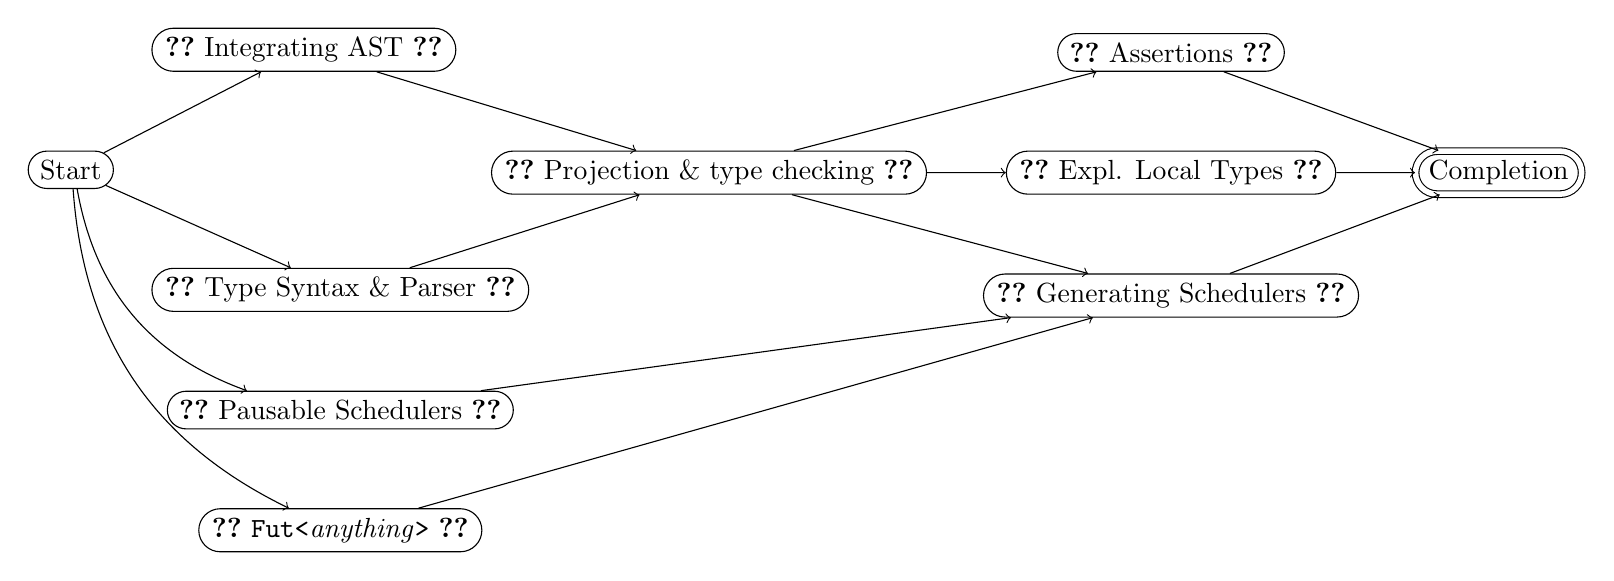
\begin{tikzpicture}
  \node (start)
        [draw, rounded rectangle]
        {Start};
  \node (syntaxAndParser)
        [draw,rounded rectangle,below right=of start]
        {\ref{WPsyntaxAndParser} Type Syntax \& Parser \ref{ordersyntaxAndParser}};
  \node (PassAST)
        [draw,rounded rectangle,above right=of start]
        {\ref{WPPassAST} Integrating AST \ref{orderPassAST}};
  \node (ProjectionAndTC)
        [draw,rounded rectangle,below right=of PassAST]
        {\ref{WPProjectionAndTC} Projection \& type checking \ref{orderProjectionAndTC}};
  \node (ExplicitTypes)
        [draw,rounded rectangle,right=of ProjectionAndTC]
        {\ref{WPExplicitTypes} Expl. Local Types \ref{orderExplicitTypes}};
  \node (Assertions)
        [draw,rounded rectangle,above=of ExplicitTypes]
        {\ref{WPAssertions} Assertions \ref{orderAssertions}};
  \node (GenSchedulers)
        [draw,rounded rectangle,below=of ExplicitTypes]
        {\ref{WPGenSchedulers} Generating Schedulers \ref{orderGenSchedulers}};
  \node (ExtendScheduler)
        [draw,rounded rectangle,below=of syntaxAndParser]
        {\ref{WPExtendScheduler} Pausable Schedulers \ref{orderExtendScheduler}};
  \node (AnyFut)
        [draw,rounded rectangle,below=of ExtendScheduler]
        {\ref{WPAnyFut} \texttt{Fut<}\emph{anything}\texttt{>} \ref{orderAnyFut}};
  \node (End)
        [draw,rounded rectangle,double,double distance=0.7mm,right=of ExplicitTypes]
        {Completion};

  \draw[->] (start) -- (syntaxAndParser);
  \draw[->] (start) -- (PassAST);
  \draw[->] (start) to[bend right] (AnyFut);
  \draw[->] (start) to[bend right] (ExtendScheduler);
  \draw[->] (syntaxAndParser) -- (ProjectionAndTC);
  \draw[->] (ProjectionAndTC) -- (ExplicitTypes);
  \draw[->] (ProjectionAndTC) -- (GenSchedulers);
  \draw[->] (ProjectionAndTC) -- (Assertions);
  \draw[->] (PassAST) -- (ProjectionAndTC);
  \draw[->] (Assertions) -- (End);
  \draw[->] (ExplicitTypes) -- (End);
  \draw[->] (GenSchedulers) -- (End);
  \draw[->] (ExtendScheduler) -- (GenSchedulers);
  \draw[->] (AnyFut) -- (GenSchedulers);
\end{tikzpicture}
}

\medskip

Based on this system of dependencies, the following implementation order has
been determined.

\begin{enumerate}[label=(\arabic*)]
  \item \label{orderExtendScheduler} \ref{WPExtendScheduler} Pausable Schedulers
  \item \label{orderAnyFut} \ref{WPAnyFut} \texttt{Fut<}\emph{anything}\texttt{>}
  \item \label{ordersyntaxAndParser} \ref{WPsyntaxAndParser} Type Syntax \& Parser
  \item \label{orderPassAST} \ref{WPPassAST} Integrating AST
  \item \label{orderProjectionAndTC} \ref{WPProjectionAndTC} Projection \& type checking
  \item \label{orderGenSchedulers} \ref{WPGenSchedulers} Generating Schedulers
  \item \label{orderExplicitTypes} \ref{WPExplicitTypes} Expl. Local Types
  \item \label{orderAssertions} \ref{WPAssertions} Assertions
\end{enumerate}

The following considerations have influenced the decided order:
\begin{itemize}
  \item \ref{WPExtendScheduler} and \ref{WPAnyFut} have been picked as first items, such that necessary changes to Core ABS can be discussed with the ABS developers early on.

    This also allows to get familiar with the internals of the ABS compiler.
  \item Since \ref{WPAssertions} is optional, it has been placed at the end of
    the list.
\end{itemize}

\paragraph{Schedule}% TODO: Kompatibilität mit Zeitplan für ABS workshop?
Available time: 26 weeks.

\medskip
%
\setdate{2019-05-08}%
\newcommand\nextdays[1]{\adddays{#1}\DTMusedate{mydate}}%
\newcommand\nextday{\nextdays{1}}%
\DTMsetstyle{ddmmyy}%
%
\begin{tabular}{llll}
Working Package & Allotted Time & Start Date & End Date \\
\hline
Pausable Schedulers & 2 weeks                                  & \DTMusedate{mydate} & \nextdays{13} \\
\texttt{Fut<}\emph{anything}\texttt{>} & 1.5 weeks             & \nextday & \nextdays{10} \\
Type Syntax \& Parser & 2 weeks                                & \nextday & \nextdays{13} \\
Integrating AST & 1.5 weeks                                    & \nextday & \nextdays{10} \\
Projection \& type checking & 5 weeks                          & \nextday & \nextdays{34} \\
Generating Schedulers (part 1) & 2.5 weeks                     & \nextday & \nextdays{17} \\
Preparation for midway presentation & 1 week                   & \nextday & \nextdays{6} \\
Generating Schedulers (part 2) & 2.5 weeks                     & \nextday & \nextdays{17} \\
Expl. Local Types & 3 weeks                                    & \nextday & \nextdays{20} \\
Assertions & 2.5 weeks                                         & \nextday & \nextdays{17} \\
Final revisions, preparation of final presentation & 2.5 weeks & \nextday & \nextdays{17}
\end{tabular}

\medskip

Increased preparation effort for exams is to be expected around the time from
the 8th of July to the 8th of August. This corresponds to about 8.5 weeks from the
start of the thesis when assuming the 8th of May as starting point.
Since around that time the working packages with the biggest time frames are
scheduled, this should provide a slight safety margin to account for the
heightened workload.

The implementation of the working package regarding generating schedulers
\ref{WPGenSchedulers} is split into two parts to accommodate for a week of
preparation for the intermediate presentation which will probably take place
around that time.

\printbibliography[heading=bibnumbered]

\end{document}

% vim: set spell spelllang=en_us
